\section{Case Study and Results}
\title{Case Study and Results}
\begin{frame}{Case Study and Results}

\begin{block}{Tennessee Eastman Process}
It is a plant wide industrial process based on an actual chemical process from the group Eastman Chemical Company. \footcite{downs1993plant}
    \begin{equation}
        \begin{matrix}
            & A(g) + C(g) + D(g) \rightarrow G(liq), & \text{Product 1} \\
            & A(g) + C(g) + E(g) \rightarrow H(liq), & \text{Product 2} \\
            & A(g) + E(g) \rightarrow F(liq), & \text{Byproduct} \\
            & 3D(g) \rightarrow 2F(g), & \text{Byproduct}
        \end{matrix}
    \label{eq:tep_react}
    \end{equation}
\end{block}
\end{frame}

\begin{frame}[c]{Case Study and Results}

    \BlankLine
    \BlankLine
    \begin{table}[!h]
        \centering
        \begin{tabular}{|c|c|}
        \hline
        \textbf{Parameters}    &  \textbf{Settings}\\
        \hline
        Simulation Time     &  760 hours \\
        \hline
        Disturbance length & 1 hour\\
        \hline
        Stabilization length & 14 hours\\
        \hline
        Disturbance &   \# 6 - A Feed Loss \\
        \hline
        Number of disturbance activation  & 50 times\\ 
        \hline
        Sampling Frequency & 100 samples per hour \\
        \hline
        \end{tabular}
    
        \caption{Experimental setup of the simulation of TEP}
        \label{tab:tepSetup}
    \end{table}
\end{frame}

\begin{frame}{Case Study and Results - Selected Variables}
\small
    \begin{table}[!h]
    \renewcommand{\arraystretch}{1.3}
    \centering
    \begin{tabular}{|c|c|}
    \hline
    \textbf{Variable} & \textbf{Description}  \\ 
    \hline
    $\mathit{x_1}$ &  A Feed ({stream 1})  \\
    \hline
    $\mathit{x_2}$ & D Feed ({stream 2}) \\
    \hline
    $\mathit{x_3}$ & E Feed ({stream 3})\\
     \hline
    $\mathit{x_6}$ &  Reactor Feed Rate (stream 6) \\
    \hline
    $\mathit{x_7}$ &  Reactor Pressure \\
    \hline
    $\mathit{x_8}$ & Reactor Level \\
    \hline
    $\mathit{x_9}$ & Reactor Temperature \\
    \hline
    $\mathit{x_{21}}$ & Cooling water  outlet temperature \\
    \hline
    \end{tabular}
    \caption{Description of process variable analyzed}
    \label{tab:varDescript}
\end{table}
\end{frame}


\begin{frame}{Case Study and Results - TEP}

\begin{figure}[!h]
    \centering
    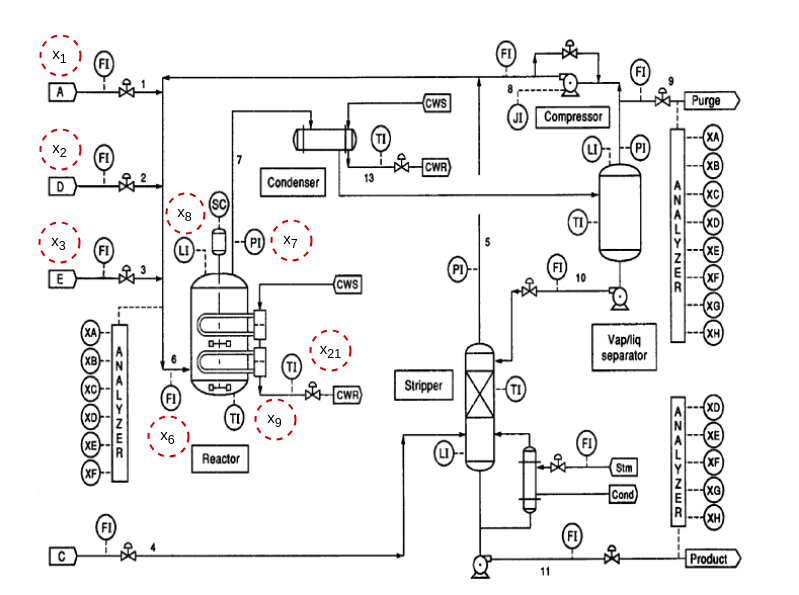
\includegraphics[keepaspectratio, width=\textwidth,height=0.7\textheight]{figuras/tep_inteiro.png}
    \caption{TEP schematic}
    \label{fig:tep}
\end{figure}
    
\end{frame}

\begin{frame}{Case Study and Results - Alarm Settings}

\begin{equation}
H_{a} = \left\{
\begin{matrix}
 1 , & V_p(t)   \geq \mu' + 3\sigma' & \\
 0,  & V_p(t)  < \mu' + 3\sigma'
\end{matrix} \right.
\label{eq:threshAlarm}
\end{equation}


\begin{equation}
    L_{a} = \left\{
    \begin{matrix}
     1 , & V_p(t)   \leq \mu' - 3\sigma' & \\
     0,  & V_p(t)  > \mu' - 3\sigma'
    \end{matrix} \right.
    \label{eq:threshAlrmLow}
    \end{equation}

\end{frame}

\begin{frame}{Case Study and Results - Processing of the Data}
\centering \textbf{Moving Mean application}

\begin{columns}

\column{0.5\textwidth}
    \begin{figure}
        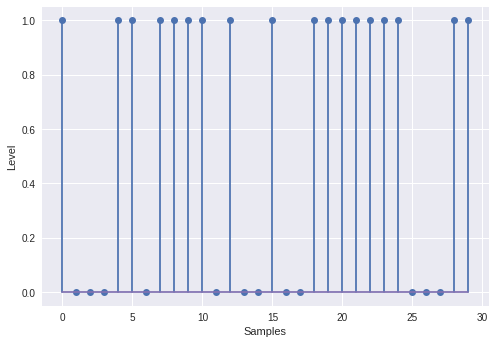
\includegraphics[scale=0.3]{figuras/signalstem.png}
        \caption{Discrete Time Signal}
        \label{fig:stem}
    \end{figure}
\column{0.5\textwidth}
    \begin{figure}
        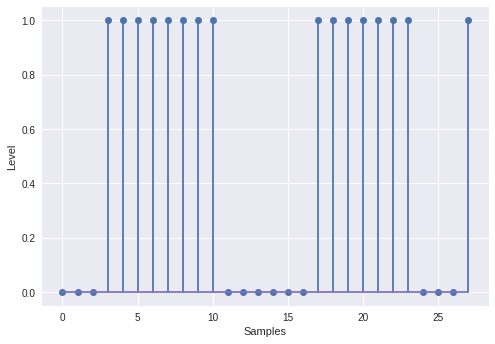
\includegraphics[scale=0.3]{figuras/stemmoving.png}
        \caption{Signal after moving average application}
        \label{fig:stem}
    \end{figure}
\end{columns}

\end{frame}




\begin{frame}{Case Study and Results}
    
\end{frame}